\documentclass[cs4size,a4paper,adobefonts]{ctexart}
\usepackage{amsmath,amsthm,amssymb}
\usepackage[colorlinks=true,allcolors=black]{hyperref}
\usepackage{indentfirst}
\usepackage[a4paper,left=2.5cm,right=2.5cm,bottom=2.5cm,top=2.5cm]{geometry}
\usepackage{graphicx}
\usepackage{subcaption}
\usepackage{url}
\usepackage{fontspec}
\setmainfont{Palatino}
\setmonofont[Scale=MatchLowercase]{Monaco}
\pagestyle{plain}
\punctstyle{kaiming}
\usepackage{unicode-math}
\setmathfont{Asana Math}

\newcommand{\GridMaze}{\href{http://itunes.apple.com/app/grid-maze/id553265800?mt=8}{Grid Maze}}
\graphicspath{{pic/}}

\begin{document}
\title{\bfseries 算法有什么用}
\author{\href{mailto:txyyss@gmail.com}{王盛颐}}
\date{}
\maketitle

\section*{缘起}
最近我的 iPad 程序 \GridMaze{} 在历经了 5 个月的开发,13 天的审核之后,
终于在苹果应用商店上架了。这个程序的主要功能是能根据输入的文字或图案,
生成一个迷宫,使得走出这个迷宫的唯一路径能形成当初输入的文字或图案。

生成这样一个迷宫的想法最早可以追溯到 2007 年底,不过那时完全不知道该怎
么做,于是这个想法也就是在脑子里徘徊了一阵,就置之一旁了。直到一年后也
就是 2008 年底,在看到一篇根据图形生成迷宫轮廓的文章
\cite{Xu:2007:ImageMaze}时,我突然想明白该怎么做了,于是就用
Mathematica 做了一些试验验证了我的想法,之后就一边完善想法一边写程序,
直到做出了一个以我名字为解法的迷宫。这个原型程序也就因为目标已达成而被
束之高阁。2010年,在朋友的鼓励下,我用 Qt 写了这个迷宫生成程序的界面,
同时用 C++ 重写了原先用 Java 和 Mathematica 写的部分,完善了一些功能,
这就是
\href{https://sites.google.com/site/txyyss/projects/text-maze-creator}{Text
  Maze Creator}。这个程序依赖一个第三方的 TSP 求解程序和一个
ActionScript 的编译器,操作起来很复杂,所以也没有提供下载,只是放了一些
样例在网上。转眼就到了2012 年,由于陆续能收到请求生成迷宫的邮件,我决定
写一个大家都能用的迷宫生成程序。我重新设计了界面,自己写了 TSP 的求解算
法,这才有了 iPad 上的 \GridMaze。

在开发 \GridMaze{} 的过程中,我遇到了很多有意思的问题,为了解决这些问题
参考和设计了很多算法。我觉得有必要把这些问题和解决办法整理一番,也算是
在初步完成这个项目之后,做一个总结报告。

\section{概述}
名不正则言不顺,言不顺则事不成。我先明确一下要解决的问题:生成一个迷宫,
使得走出这个迷宫的唯一路径能形成指定的文字或图案。这句话不够精确,需要
进一步的解释来消除歧义。

首先是“迷宫”的意思。本文的迷宫专指一种需要玩家从一个指定的起点出发,在
用墙隔断形成的分叉道路中辨识选择,最终到达指定终点的游戏。这样的迷宫具
有很多种形式(图 \ref{fig:manyMazes}),我要生成的迷宫是外轮廓为矩形,
分叉道路横平竖直,每一段墙的长度为单位长度整数倍的,解法唯一的所谓“标准
迷宫”(图 \ref{fig:rectMaze})。

\begin{figure}[htbp]
  \centering
  \begin{subfigure}[c]{0.31\textwidth}
    \centering
    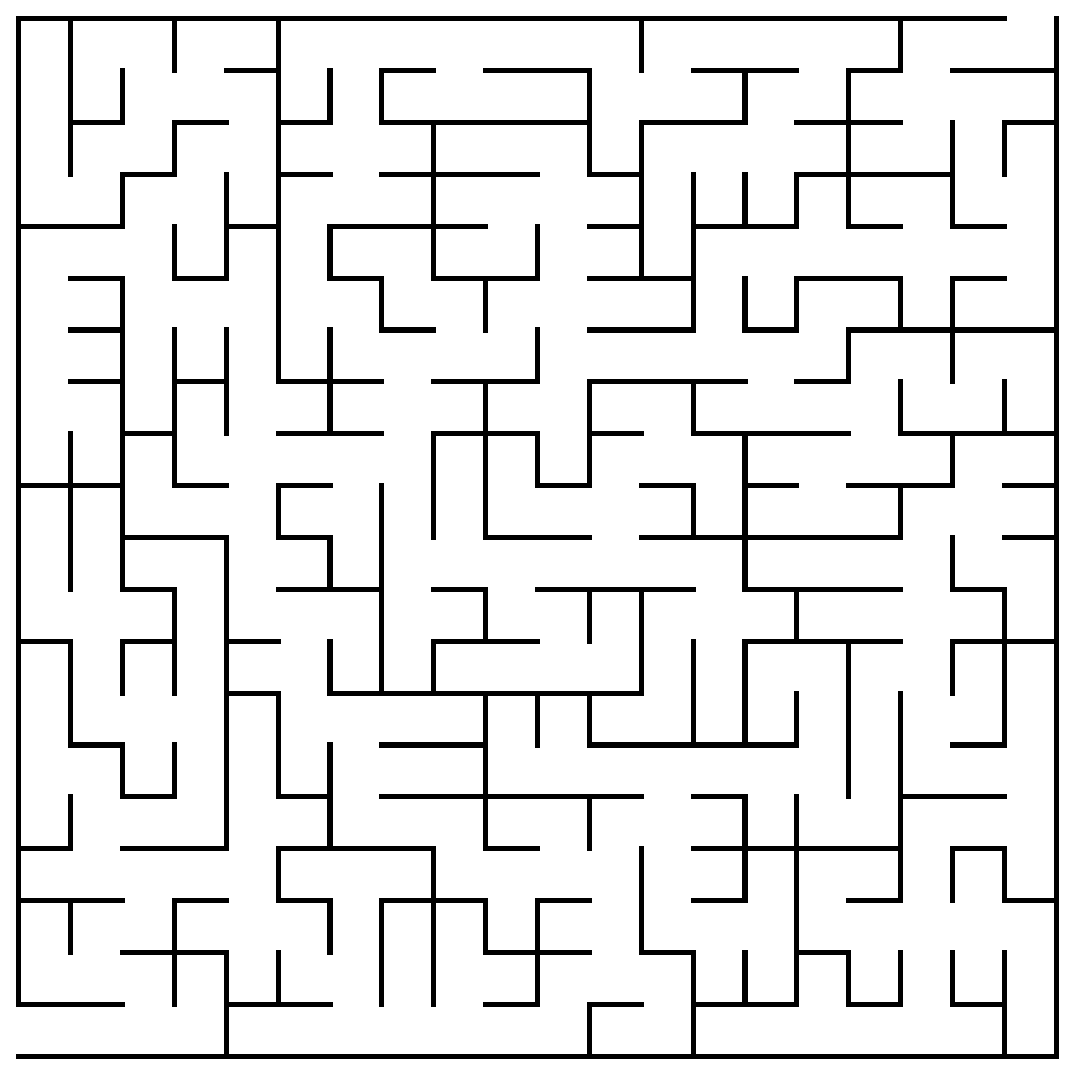
\includegraphics[width=\textwidth]{rectMaze}
    \caption{标准迷宫}\label{fig:rectMaze}
  \end{subfigure}
  ~
  \begin{subfigure}[c]{0.31\textwidth}
    \centering
    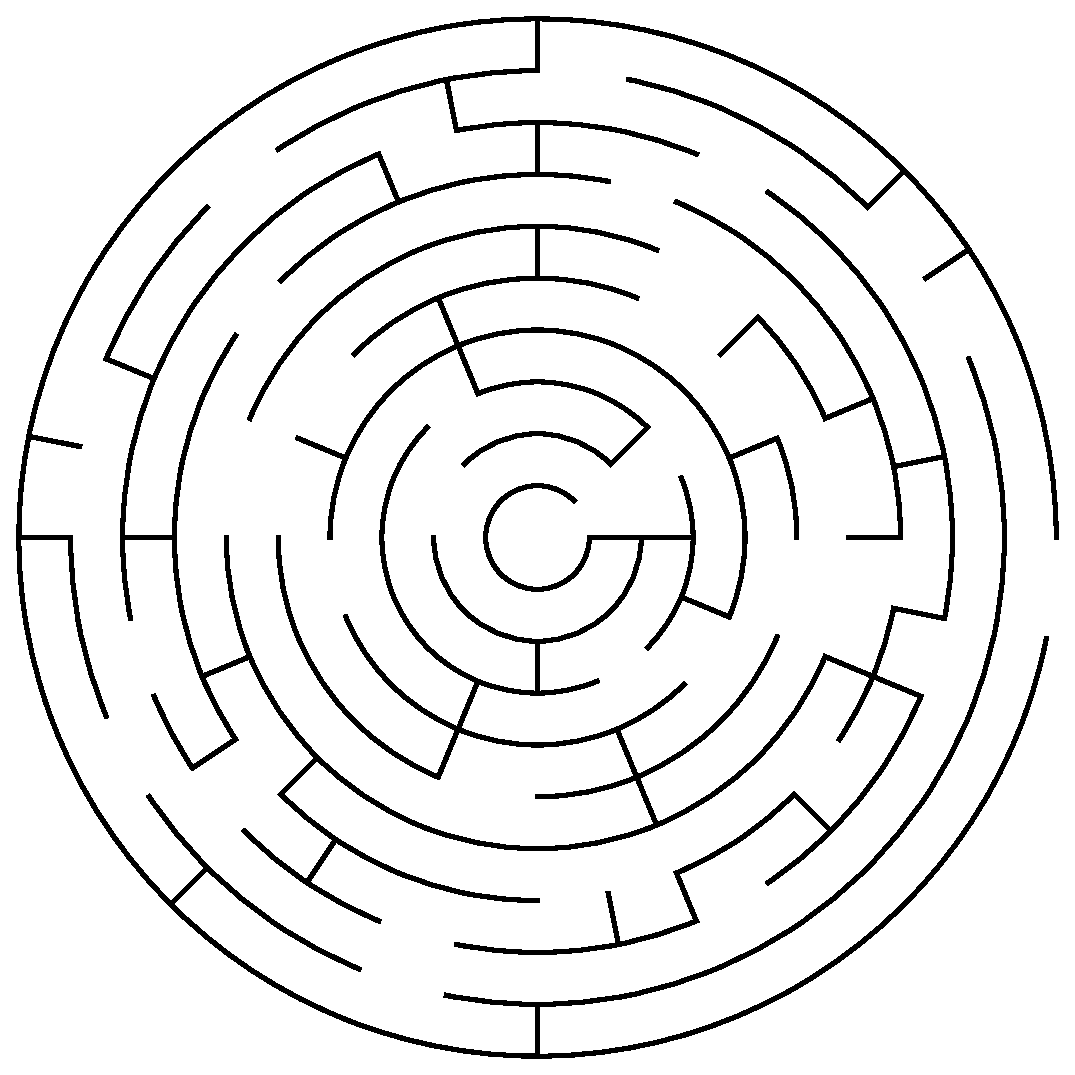
\includegraphics[width=\textwidth]{diskMaze}
    \caption{圆形迷宫}\label{fig:diskMaze}
  \end{subfigure}
  ~
  \begin{subfigure}[c]{0.31\textwidth}
    \centering
    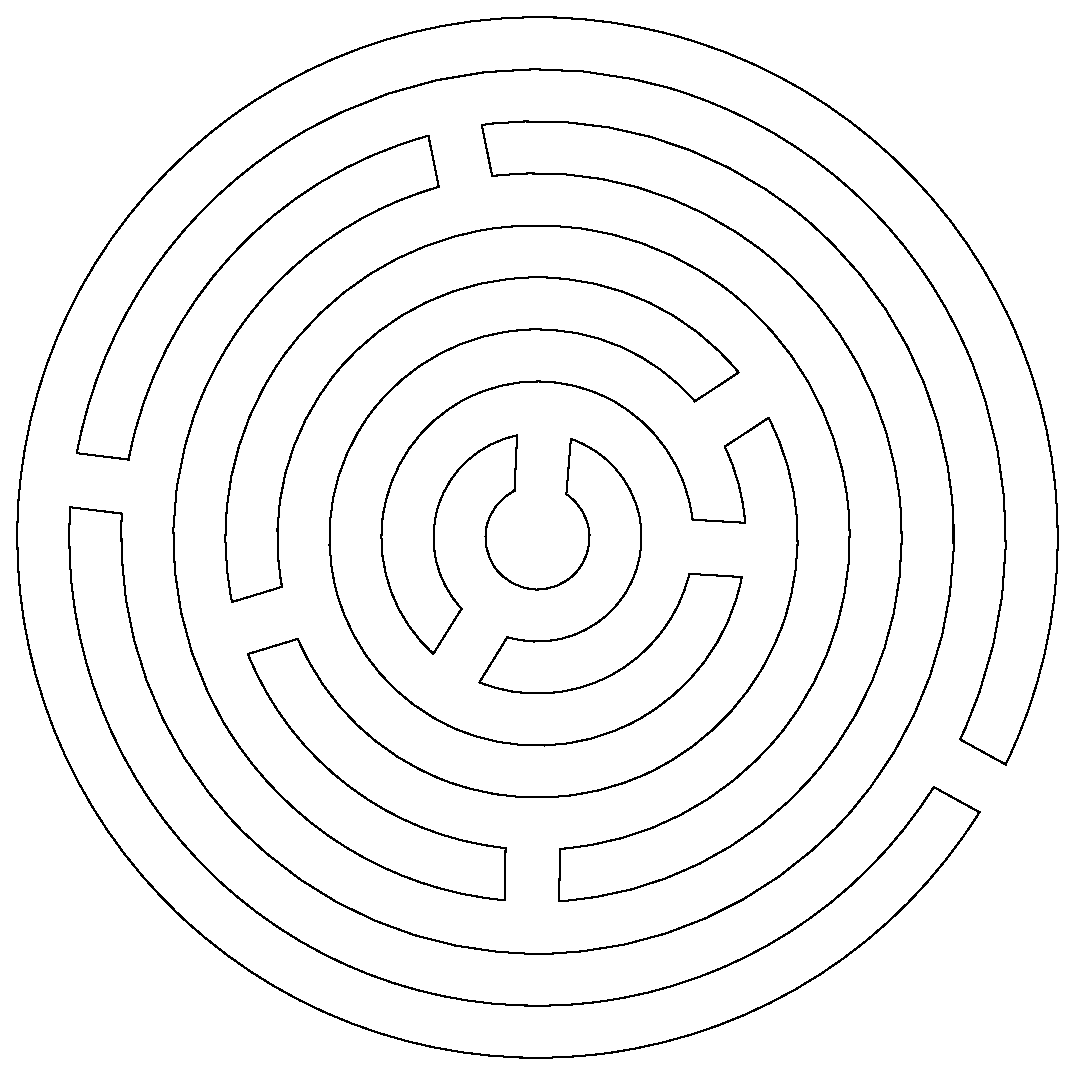
\includegraphics[width=\textwidth]{eulerMaze}
    \caption{一笔画迷宫}
  \end{subfigure}
  \caption{各种不同类型的迷宫}\label{fig:manyMazes}
\end{figure}

接下来定义什么叫“路径形成指定的文字或图案”。我将文字或图案变成点阵(如
  图 \ref{fig:abcGrid}),如果有条路径能把这个点阵串起来,并且这条路径
上只遗漏了少量点阵中的点,只增加了少量不在这个点阵中的点。那么就可以说
路径形成了指定的文字或图案(如图 \ref{fig:abcPath})。当然,由于这条路
径还要是“标准迷宫”的解答路径,所以还必须加上横平竖直,自身无交叉两个额
外的条件。

\begin{figure}[htbp]
  \centering
  \begin{minipage}{0.5\textwidth}
    \centering
    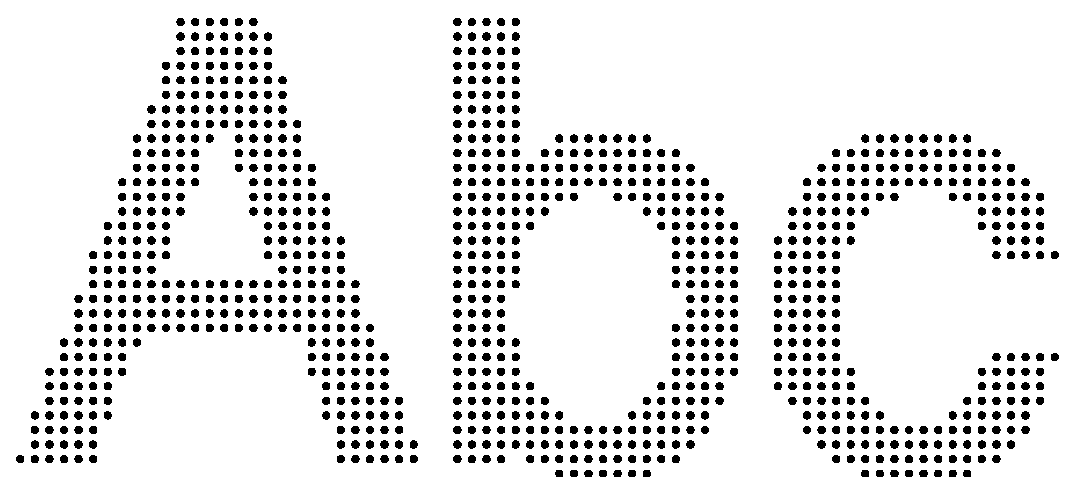
\includegraphics[width=0.95\linewidth]{abcGrid}
    \caption{文字点阵}\label{fig:abcGrid}
  \end{minipage}%
  \begin{minipage}{0.5\textwidth}
    \centering
    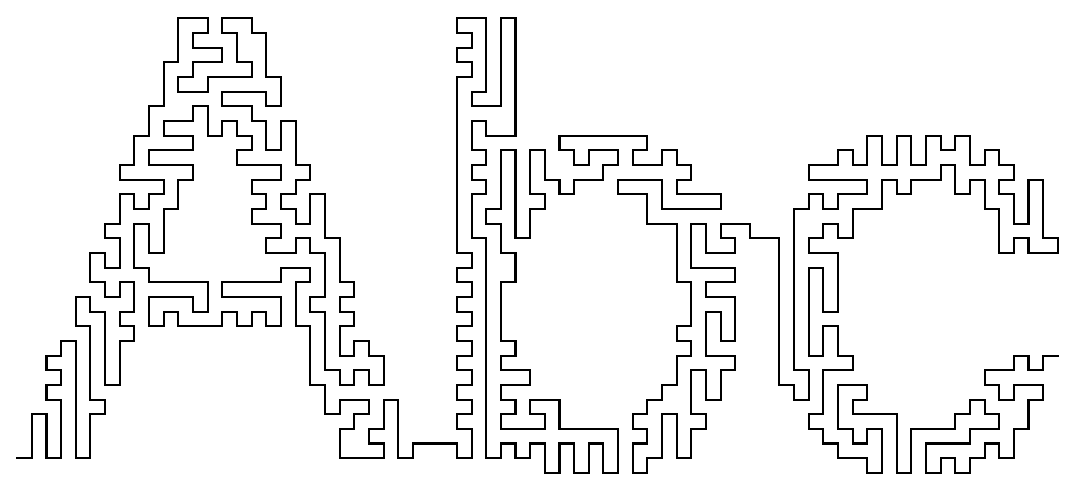
\includegraphics[width=0.95\linewidth]{abcPath}
    \caption{路径形成的文字}\label{fig:abcPath}
  \end{minipage}
\end{figure}

在明确了这两点之后,要解决的问题就清楚了。首先要根据点阵生成解答路径,
其次要根据解答路径生成迷宫。通过进一步的思考我发现,生成路径这个问题比
生成迷宫要困难得多。本着先易后难的原则,下面我先介绍如何根据已有的解答
路径,生成迷宫。

\section{迷宫生成算法}
生成迷宫有许多种算法 \cite{wiki:mazeGen}。我用的是基于图论的生成方法。
从一组预先安排好的互相隔断的格子布局开始,从这布局可以定义一个无向图
$G=(V,E)$,结点集合 $V$ 就是全部的格子,边的集合 $E$ 定义如下:若格子
$a,b$ 位于一堵墙的两侧,则 $\{a,b\}\in E$。

对任意 $F\subset E$,图 $G$ 的子图 $S=(V,F)$ 都对应一个迷宫,反之亦然。
具体对应方法如下:在原来布局的基础上,若 $e\in F$,则拆掉边 $e$ 对应的
那堵墙,也就是说 $S$ 的边意味着迷宫的通路。若 $S$ 不连通,那意味着对应
的迷宫有格子不可达,这显然不够理想。若 $S$ 中出现环路,则意味着迷宫的求
解路径可能不止一条,这也不理想。所以一个理想的迷宫对应的子图 $S$ 全连通
且无环,这正是图 $G$ 的支撑树 (Spanning Tree)。

\begin{figure}[htbp]
  \centering
  \begin{subfigure}[c]{0.31\textwidth}
    \centering
    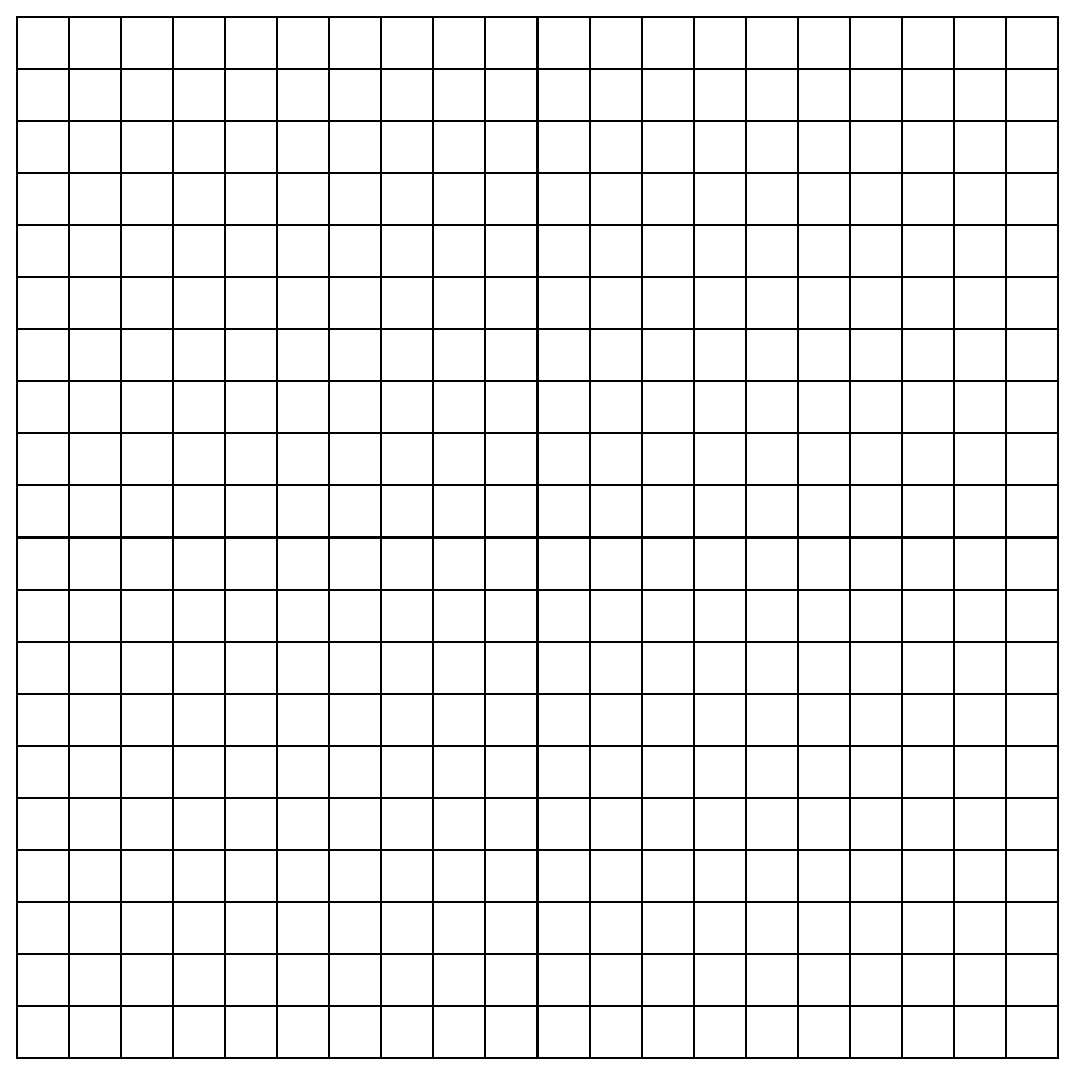
\includegraphics[width=\textwidth]{rectCells}
    \caption{标准迷宫的格子布局}
  \end{subfigure}
  ~
  \begin{subfigure}[c]{0.31\textwidth}
    \centering
    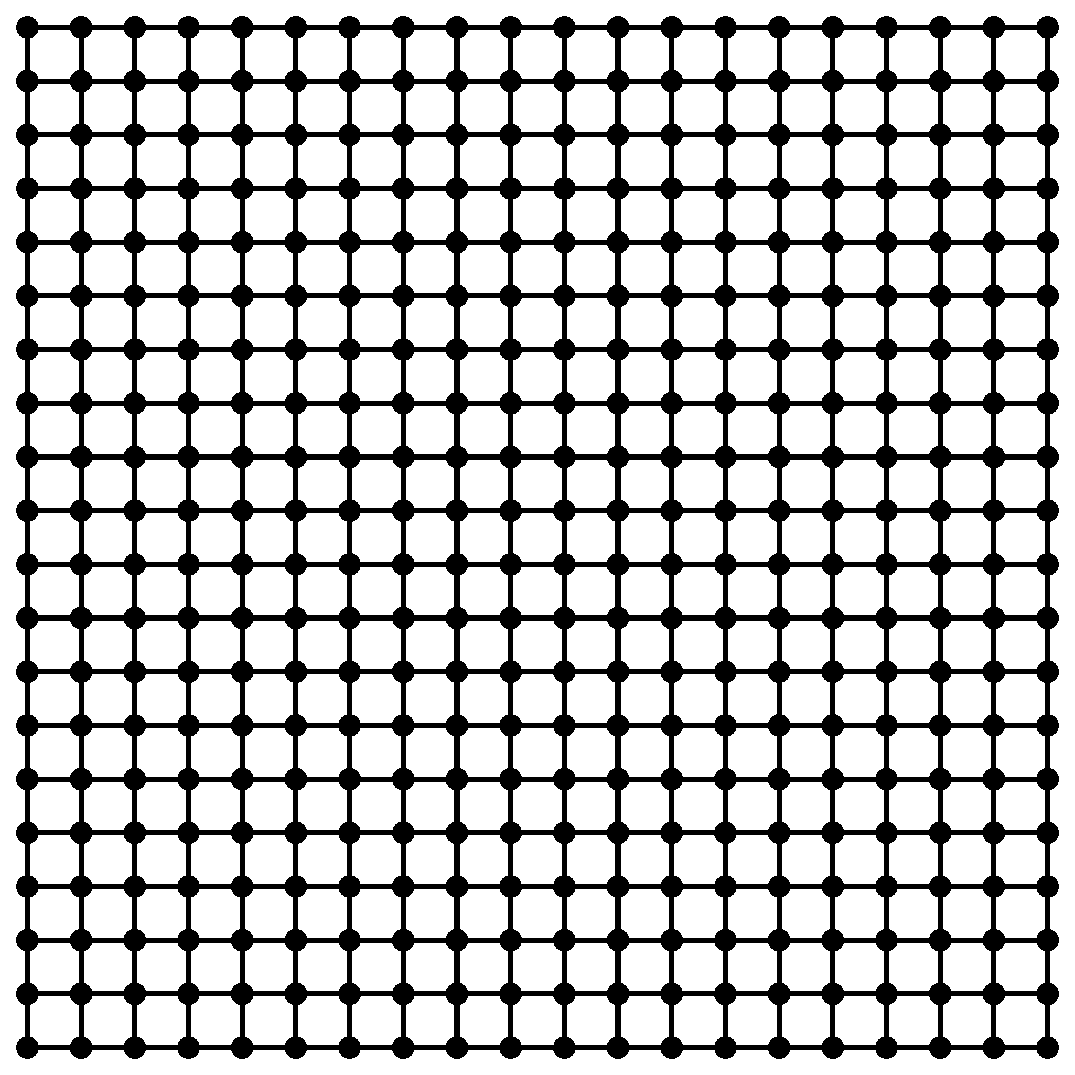
\includegraphics[width=\textwidth]{rectGraph}
    \caption{布局对应的无向图 $G$}
  \end{subfigure}
  ~
  \begin{subfigure}[c]{0.31\textwidth}
    \centering
    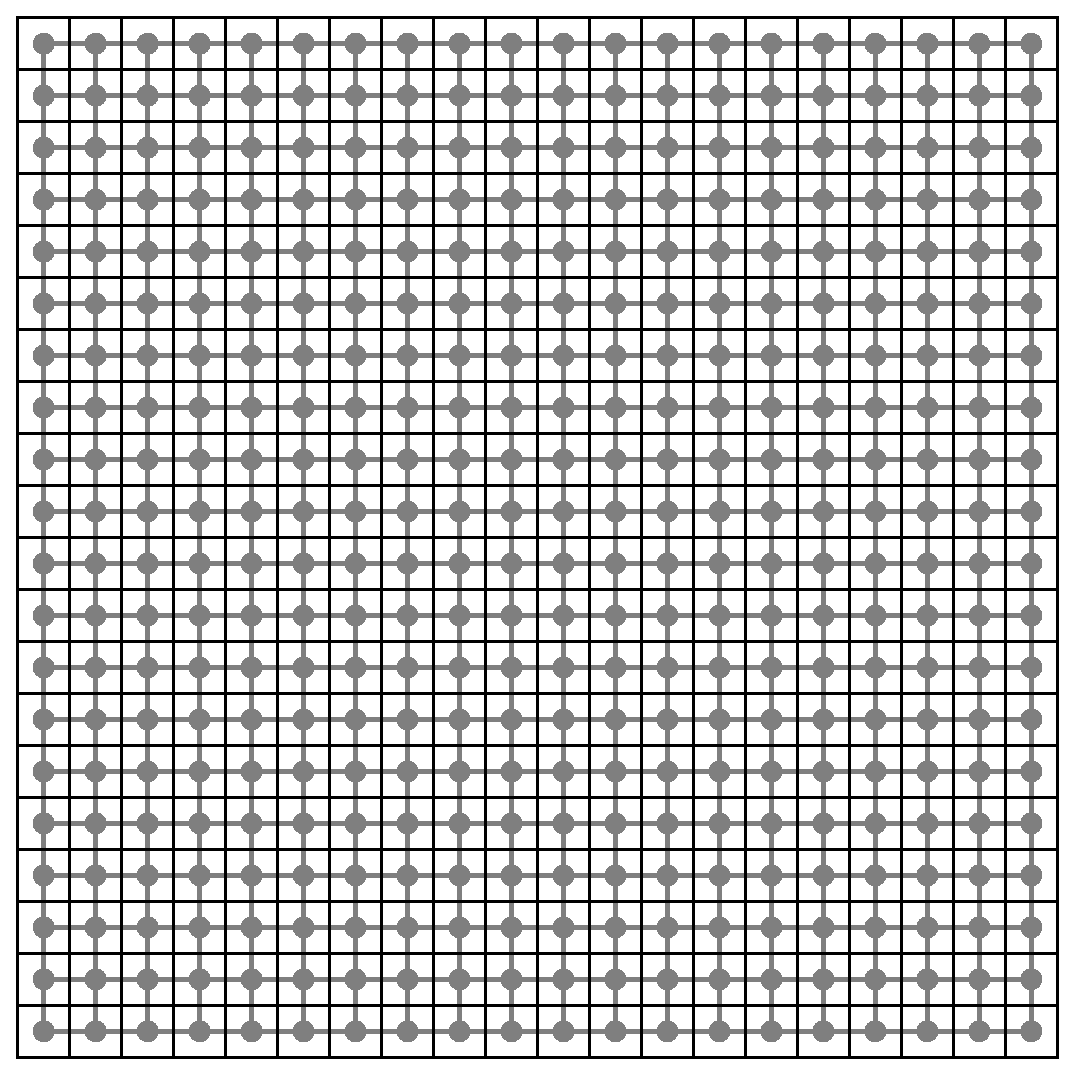
\includegraphics[width=\textwidth]{rectMerged}
    \caption{将布局和图合并在一起}
  \end{subfigure}
  \caption{标准迷宫的布局和由它定义的无向图}\label{fig:rectMazeGen}
\end{figure}

到这里一个普通迷宫的生成算法就很显然了,任意计算支撑树的算法都可以。比
如随机 Kruskal 算法:
\begin{enumerate}
\item 创建一个全部墙的列表 $l$,给每个格子创建一个集合,该集合开始只包
  含那个格子一个元素
\item 乱序遍历 $l$,遍历时做如下操作:
  \begin{itemize}
  \item 若墙两边的格子属于一个集合,则不做任何操作
  \item 若强两边的格子不在一个集合里,则拆除这堵墙,合并两边格子所在的集合
  \end{itemize}
\end{enumerate}

\begin{figure}[htbp]
  \centering
  \begin{subfigure}[c]{0.31\textwidth}
    \centering
    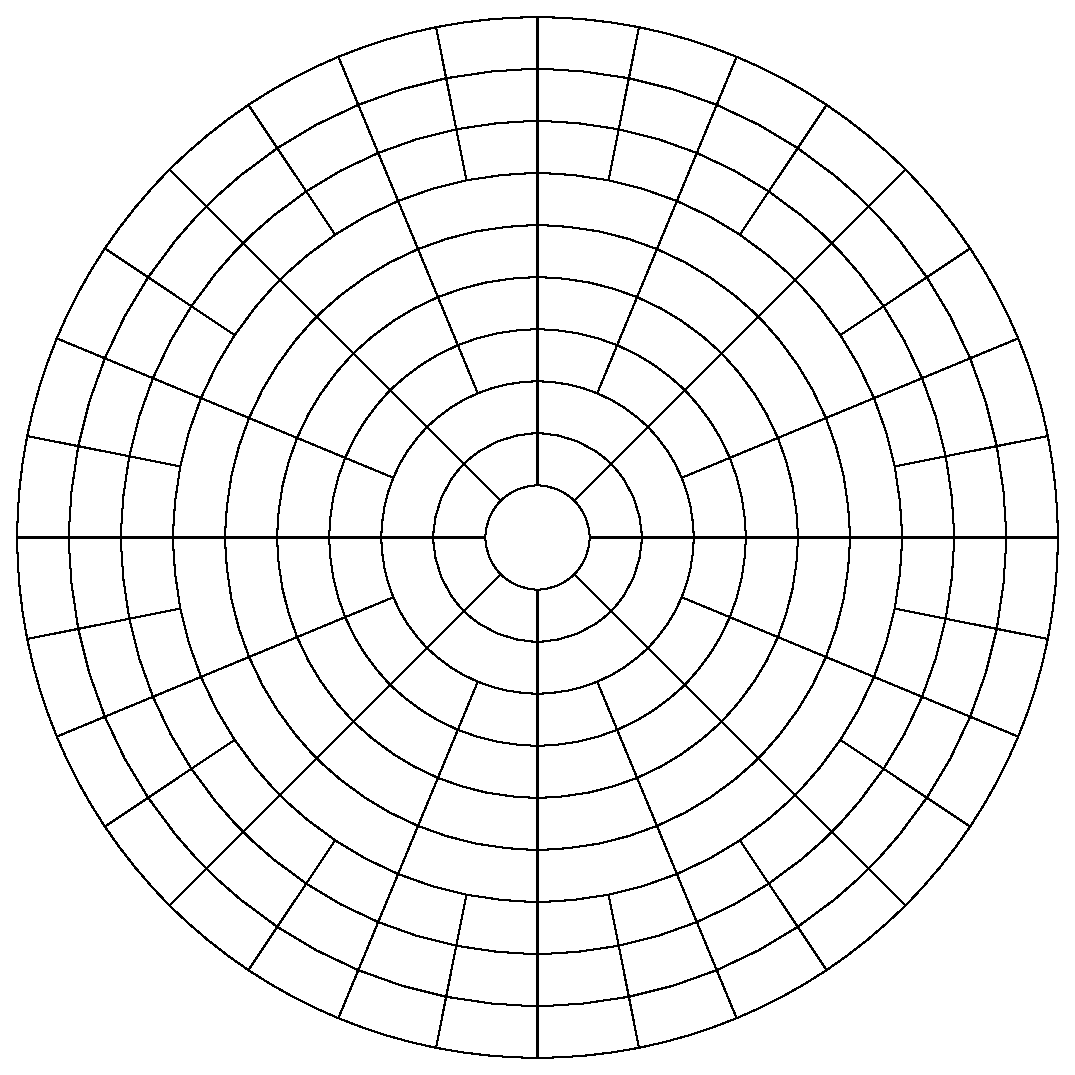
\includegraphics[width=\textwidth]{diskCells}
    \caption{圆形迷宫的格子布局}
  \end{subfigure}
  ~
  \begin{subfigure}[c]{0.31\textwidth}
    \centering
    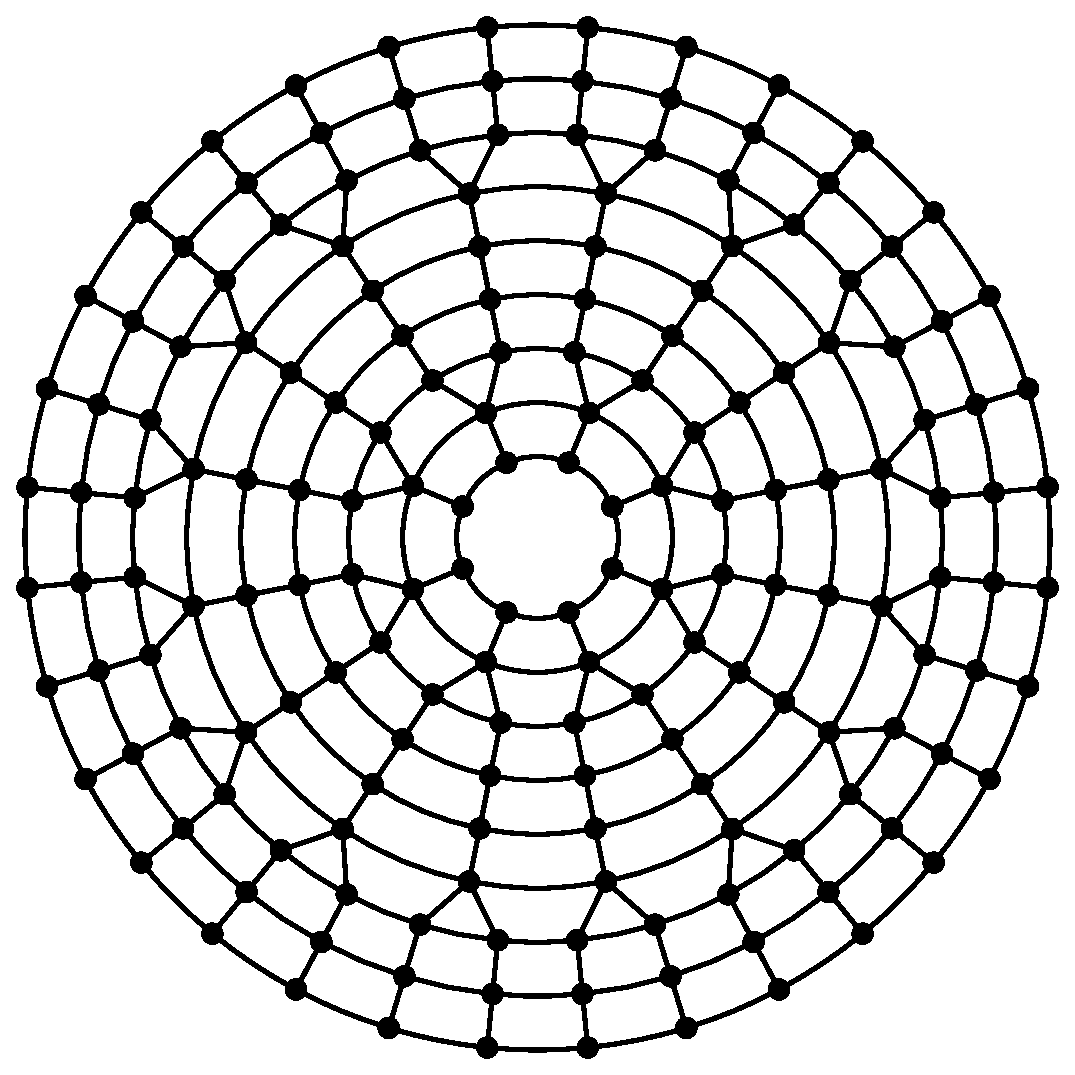
\includegraphics[width=\textwidth]{diskGraph}
    \caption{布局对应的无向图 $G$}
  \end{subfigure}
  ~
  \begin{subfigure}[c]{0.31\textwidth}
    \centering
    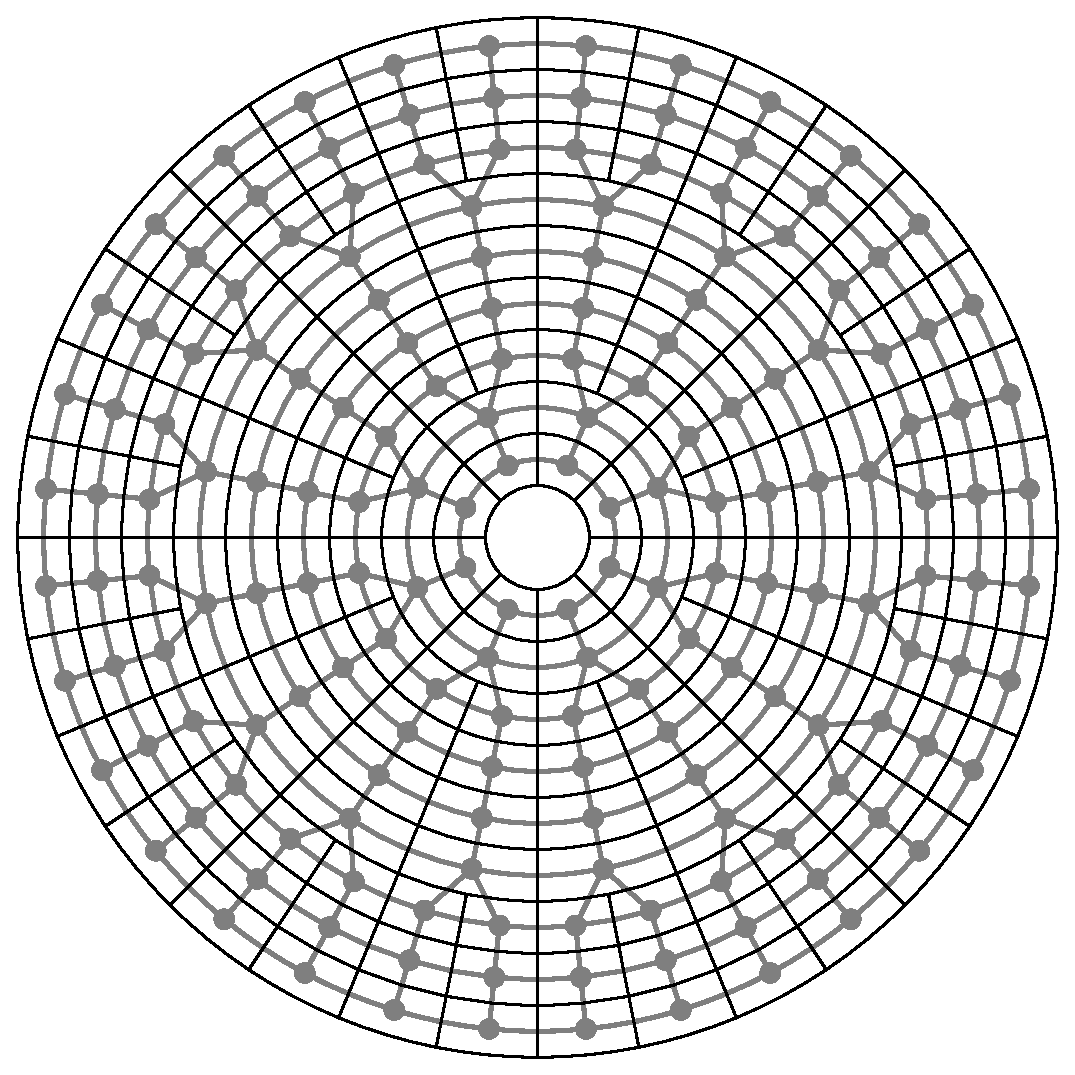
\includegraphics[width=\textwidth]{diskMerged}
    \caption{将布局和图合并在一起}
  \end{subfigure}
  \caption{圆形迷宫的布局和由它定义的无向图}\label{fig:diskMazeGen}
\end{figure}

图 \ref{fig:rectMaze} 中的标准迷宫和图 \ref{fig:diskMaze} 中的圆形迷宫
都是用随机 Kruskal 算法分别根据图 \ref{fig:rectMazeGen} 和图
\ref{fig:diskMazeGen} 中的布局生成的。有了这个算法,根据已有解答路径生
成迷宫变得轻而易举。只要把算法中 $l$ 的遍历顺序修改一下,先遍历解答路径
经过的那些墙,而后乱序遍历即可。

值得一提的是,随机 Kruskal 算法中,大量需要进行集合查找和集合合并的操作,
且这些集合彼此不相交。这可以用一种叫并查集 (Disjoint Sets) 的数据结构来
进行。这种数据结构单步进行查找或合并操作的时间复杂度几乎是常数,所以用
了这一数据结构的随机 Kruskal 算法的时间复杂度是 $O(n)$ 的,$n$ 是墙的数
量。关于 Disjoint Set 这里就不细说了,有兴趣的读者可查阅 \cite{clrs} 的
第 21 章。

\section{点阵连成路径的算法}
和生成迷宫相比,把点阵连成不自交的,横平竖直的路径要困难得多。

\bibliographystyle{unsrt}
\bibliography{algorithm}
\end{document}
